\documentclass[10pt,a4paper]{article}

% ==============================================================================
% EXPERIMENT 05: PRINTABLE SOURCE CODE & OUTPUT (EXACT SINGLE 1-PAGE DOCUMENT)
% Formatted with 1.0-inch lateral margins, large readable fonts, and tight top/bottom margins.
% ==============================================================================
\usepackage[utf8]{inputenc}
\usepackage[T1]{fontenc}
\usepackage{lmodern}
\usepackage[left=1.0in, right=1.0in, top=0.32in, bottom=0.32in]{geometry}
\usepackage{amsmath,amssymb}
\usepackage{xcolor}
\usepackage{listings}
\usepackage{graphicx}
\usepackage{booktabs}
\usepackage{tabularx}
\usepackage{titlesec}
\usepackage{caption}
\usepackage{microtype}
\usepackage{float}

% Disable all running headers, footers, and page numbers for clean print & paste
\pagestyle{empty}
\setlength{\parindent}{0pt}

% Section Titles Formatting (Enlarged)
\titleformat{\section}
  {\normalfont\normalsize\bfseries\raggedright}{\thesection}{0.5em}{}[\titlerule]

\titlespacing*{\section}{0pt}{4pt}{2pt}

% Code Listing Styling (Strict Monochrome with Enlarged Font for High-Contrast Print)
\lstdefinestyle{bwArduino}{
    language=C++,
    basicstyle=\ttfamily\scriptsize,
    keywordstyle=\bfseries,
    commentstyle=\itshape,
    stringstyle=\ttfamily,
    numbers=left,
    numberstyle=\tiny,
    numbersep=6pt,
    stepnumber=1,
    breaklines=true,
    breakatwhitespace=true,
    frame=single,
    rulecolor=\color{black},
    tabsize=2,
    showstringspaces=false,
    columns=fullflexible,
    keepspaces=true,
    lineskip=-0.3pt,
    aboveskip=2pt,
    belowskip=2pt
}

\lstdefinestyle{bwTerminal}{
    basicstyle=\ttfamily\scriptsize,
    numbers=none,
    breaklines=true,
    breakatwhitespace=true,
    frame=single,
    rulecolor=\color{black},
    columns=fullflexible,
    keepspaces=true,
    lineskip=0.4pt,
    aboveskip=1.5pt,
    belowskip=1.5pt
}

\captionsetup{font=small,labelfont=bf,skip=2pt}

\begin{document}

% ==============================================================================
% DOCUMENT HEADER
% ==============================================================================
\begin{center}
    {\large\bfseries Experiment 05: Interfacing Soil Moisture Sensor with Arduino UNO}\\[0.08cm]
    {\normalsize\textbf{Analog Resistive Sensing \& Threshold Actuation --- Program Source Code \& Experimental Output}}
\end{center}
\vspace{-0.20cm}
\rule{\textwidth}{0.9pt}
\vspace{0.04cm}

% ==============================================================================
% 1. PROGRAM SOURCE CODE
% ==============================================================================
\section*{1. Arduino C++ Source Code}

\begin{lstlisting}[style=bwArduino, title={\textbf{Listing 5.1: Microcontroller Firmware for Soil Moisture Telemetry and Threshold Actuation.}}]
/* Experiment 05: Soil Moisture Sensor Interfacing with Arduino UNO
 * Hardware Pin Connections: HW-103 Module A0 -> Pin A0 | Alert LED -> Pin 13 | VCC/GND -> 5V/GND
 * Operating Logic: ADC Value < 500 indicates DRY soil (Triggers Pin 13 LED ON) */
const int sensorPin = A0;  // Soil moisture sensor connected to Pin A0
const int ledPin = 13;     // Status LED connected to digital pin 13
int sensorValue = 0;       // Variable to store raw analog sensor value
void setup() {
  pinMode(ledPin, OUTPUT); // Configure Pin 13 as digital output driver
  Serial.begin(9600);      // Initialize UART Serial Interface at 9600 Baud
}
void loop() {
  sensorValue = analogRead(sensorPin); // Acquire 10-bit analog voltage from sensor
  Serial.print("Soil moisture Level: ");
  Serial.println(sensorValue);
  // Closed-loop threshold decision: Turn ON indicator if soil is dry
  if (sensorValue < 500) {
    digitalWrite(ledPin, HIGH); // Dry soil condition: Alert / Pump ON
  } else {
    digitalWrite(ledPin, LOW);  // Sufficient moisture: LED OFF
  }
  delay(1000); // 1-second sampling period
}
\end{lstlisting}

\vspace{0.04cm}

% ==============================================================================
% 2. EXPERIMENTAL OUTPUT & SERIAL TELEMETRY (SERIAL ORDER: 2.A -> 2.B -> 2.C)
% ==============================================================================
\section*{2. Experimental Output, Serial Monitor Telemetry \& Plotter Response}

\noindent
\textbf{A. Soil Moisture Calibration \& Observation Log:}\par\vspace{0.06cm}
{\footnotesize
\setlength{\tabcolsep}{4.2pt}
\renewcommand{\arraystretch}{1.18}
\begin{tabularx}{\textwidth}{|c|p{4.8cm}|c|c|X|}
\hline
\textbf{\#} & \textbf{Soil Medium Condition} & \textbf{ADC (0--1023)} & \textbf{Voltage} & \textbf{Indicator LED 13 Status} \\
\hline
1 & Ambient Air (Open Circuit) & $33$ & $0.16\,\text{V}$ & \textbf{ON} (Dry Soil Alarm Triggered) \\
2 & Dry Soil Specimen & $29$ & $0.14\,\text{V}$ & \textbf{ON} (Dry Soil Alarm Triggered) \\
3 & Dry Soil Specimen (Replicate) & $35$ & $0.17\,\text{V}$ & \textbf{ON} (Dry Soil Alarm Triggered) \\
4 & Moderately Moistened Soil & $560$ & $2.74\,\text{V}$ & \textbf{OFF} (Moisture Setpoint Satisfied) \\
5 & Water-Saturated Soil & $820$ & $4.01\,\text{V}$ & \textbf{OFF} (Maximum Conductivity) \\
\hline
\end{tabularx}
}

\vspace{0.22cm}

\noindent
\textbf{B. Serial Monitor Stream (9600 Baud):}\par\vspace{0.05cm}
\begin{lstlisting}[style=bwTerminal]
Soil moisture Level: 33
Soil moisture Level: 29
Soil moisture Level: 35
Soil moisture Level: 38
\end{lstlisting}

\vspace{0.20cm}

\noindent
\textbf{C. Arduino Serial Plotter Waveform Response:}\par\vspace{0.05cm}
{\centering
\fbox{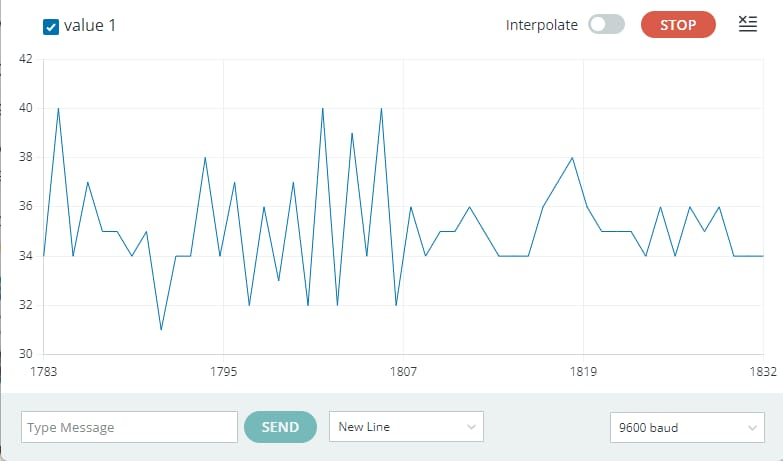
\includegraphics[width=12.8cm, keepaspectratio]{exp05_serial_plotter.jpeg}}\par\vspace{0.06cm}
{\small\textbf{Figure 5.1:} Arduino Serial Plotter waveform during dry soil baseline testing ($31 \le \text{ADC} \le 40$).}\par}

\end{document}
